\documentclass[compress,clock,xcolor=dvipsnames,hyperref={pdfpagelabels=false},final]{beamer}
\let\Tiny=\tiny
\usepackage{lmodern}
\mode<presentation>
{
 \usetheme{Warsaw}
  \setbeamercovered{transparent}
%\usecolortheme{lily}
\useoutertheme[subsection=false]{smoothbars}
\useinnertheme{rounded}
 \beamersetaveragebackground{green!10}

%\usecolortheme[named=Green]{structure}
\usecolortheme[named=OliveGreen]{structure} 
\setbeamertemplate{items}[ball] 
\setbeamercolor{structure}{fg=OliveGreen!120} 
\setbeamertemplate{blocks}[rounded][shadow=true] 
%\usecolortheme{}
}
\usepackage{graphicx} 
\usepackage{multicol}
\usepackage{hyperref}
\usepackage[utf8x]{inputenc}
\usepackage[T1]{fontenc}
\usepackage[english,polish]{babel}
\usepackage{polski}

\title[] 
{Mechanizmy wykrywania i zapobiegania przedwczesnym kodonom STOP}

\author{Małgorzata Grabińska}
\institute
{
  Zakład Genomiki, Wydział Biotechnologii\\
  Uniwersytet Wrocławski\\
{\it malgorzata.grabinska@smorfland.uni.wroc.pl}

}
\date{\today}
\AtBeginSubsection[]
{
  \begin{frame}<beamer>{Plan prezentacji}
    \tableofcontents[currentsection,currentsubsection]
  \end{frame}
}


\begin{document}

\begin{frame}[plain]

  \titlepage

\end{frame}


\section{Wprowadzenie}

%slajd 1
\begin{frame}{Przedwczesne kodony STOP (PTCs-premature STOP codons)}
\pause
\begin{itemize}
\item są wynikiem błędów powstałych w wyniku replikacji, translacji a przede wszystkim
transkrypcji;
\pause \item najczęstszymi błędami są mutacje punktowe i przesunięcia ramek odczytu;
\pause \item utworzone PTC może być dziedziczone i prowadzić do różnych chorób genetycznych, 
np. dystrofia mięśniowa Duchenna;
\pause \item PTC może prowadzić także do utraty funkcjonalności sekwencji lub 
produkcji cytotoksyn.
\end{itemize} 
\end{frame}

%slajd 2
\begin{frame}{Mechanizmy wykrywania i zapobiegania PTC}
\begin{enumerate}
\pause \item NMD (nonsense mediated decay) zjawisko występujące \\u większości eukariotów;
\pause \item używalność kodonów bezpiecznych.
\end{enumerate}
\pause
\begin{block}{cel}
 Jak organizmy prokariotyczne zapobiegają PTC?
\end{block}
\end{frame}

%slajd 3
\begin{frame}
\begin{block}{NMD}
zjawisko zachodzące w komórkach eukariotycznych , polegające na rozpoznawaniu i niszczeniu mRNA zawierający
PTC. Jest to proces kontroli jakości, zapobiega powstawaniu skróconych białek, które mogą być szkodliwe dla komórki.
\end{block}
\pause
\begin{itemize}
 \item NMD-EJC (połączenie egzon-egzon zależne od introna);
\pause \item NMD-PABP (wymaga występowania PABP-polyA niezależnego od introna).
\end{itemize}
\end{frame}

%slajd 4
\begin{frame}
\begin{columns}
 \begin{column}{0.49\textwidth}
  \scalebox{0.4}{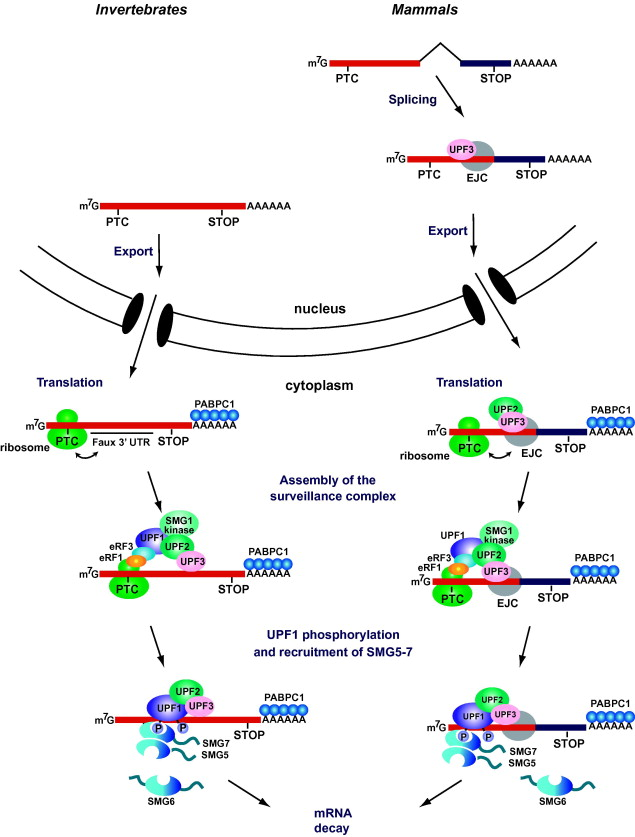
\includegraphics{rys1.jpg}}
 \end{column}
 \begin{column}{0.49\textwidth}
\center{ Rys.1. Ścieżka NMD}\\
  \tiny{,,mRNA quality control: An ancient machinery recognizes and degrades mRNAs with nonsense codon''\\
I.~Behm-Ansmant i współ.,2007, {\it  FEBS Letters} 581, 2845-2853}
 \end{column}
\end{columns}
\end{frame}

%slajd 5
\begin{frame}{Kodony ,,kruche'', ryzykowne}
\begin{center}
\scalebox{0.35}{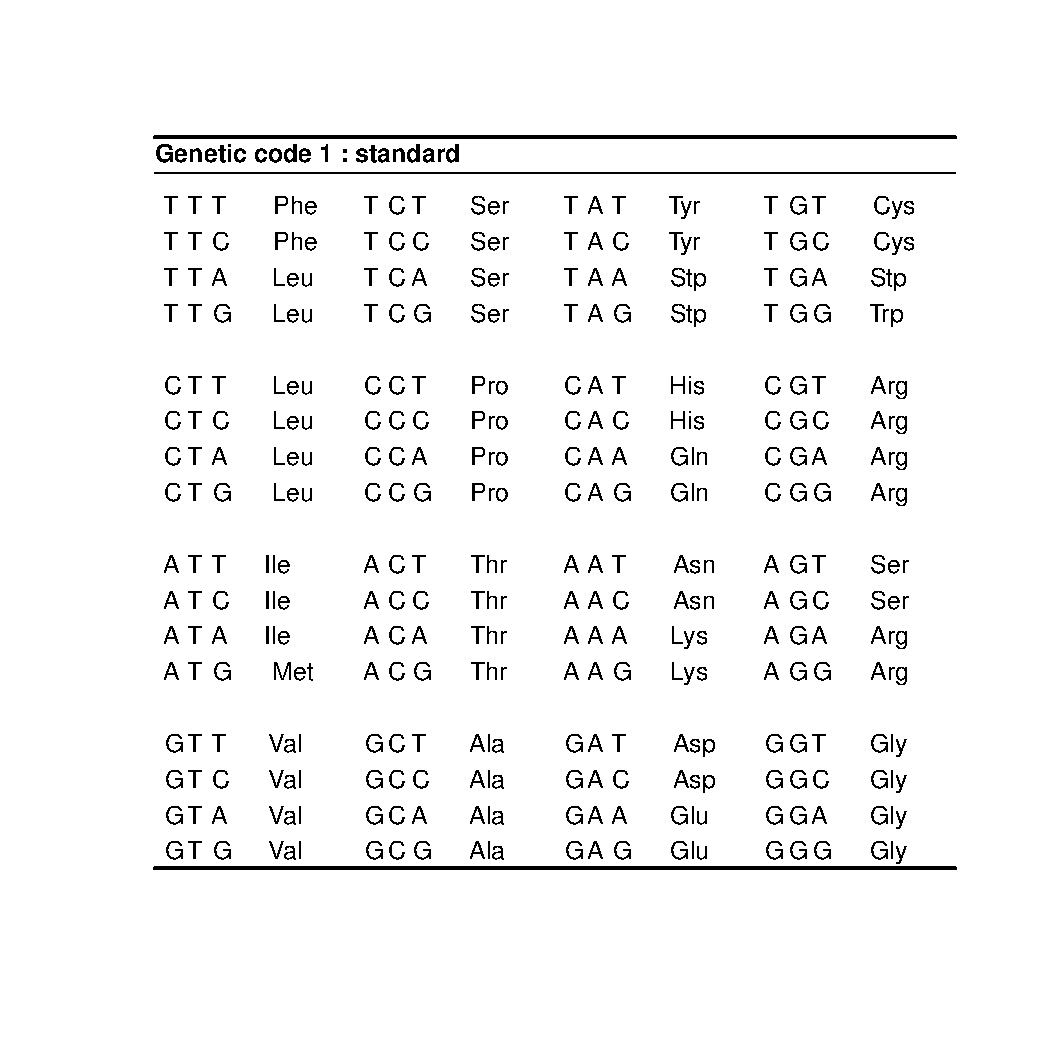
\includegraphics{rys3.pdf}}\\
\small{Tabela.1 Tabela standardowego kodu genetycznego z pakietu {\it seqinr}}
\end{center}
\end{frame}

%slajd 6
\begin{frame}{Kodony ,,kruche'', ryzykowne}
\begin{center}
\scalebox{0.35}{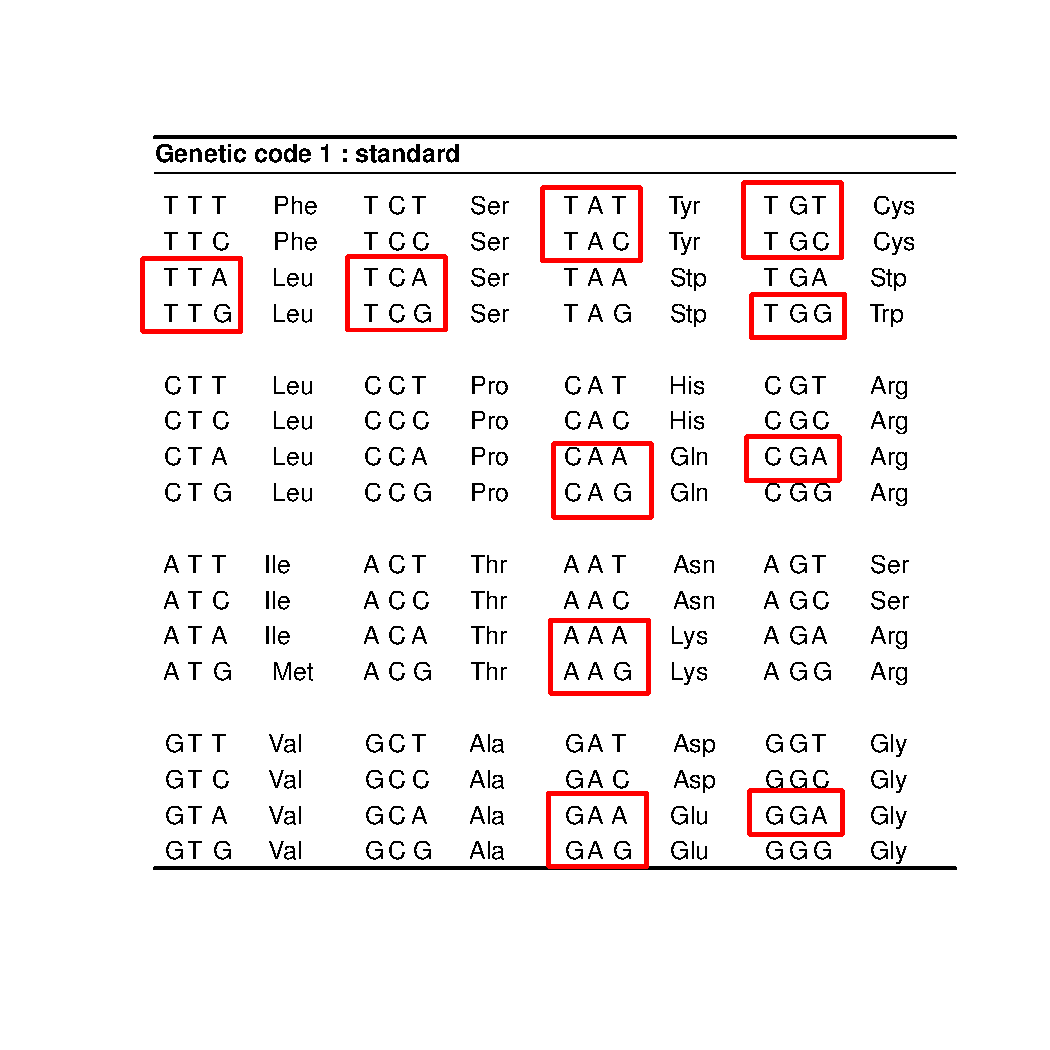
\includegraphics{rys4.pdf}}\\
\small{Tabela.2 Tabela standardowego kodu genetycznego z pakietu {\it seqinr} \\z ryzykownymi kodonami}
\end{center}
\end{frame}

%slajd 7
\begin{frame}{Kodony ,,kruche'', ryzykowne}
\begin{center}
\scalebox{0.35}{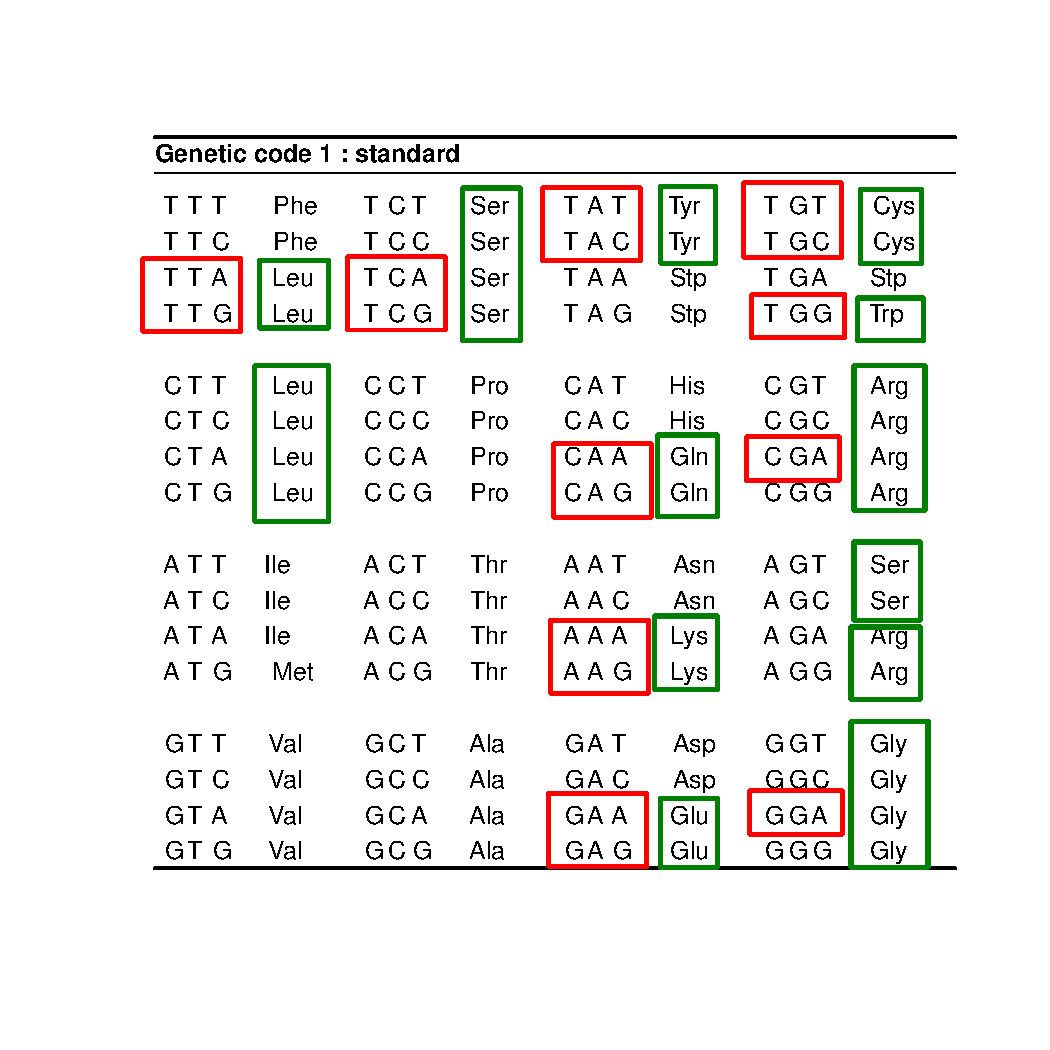
\includegraphics{rys5.pdf}}\\
\small{Tabela.3 Tabela standardowego kodu genetycznego z pakietu {\it seqinr} \\z ryzykownymi kodonami i aminokwasami}
\end{center}
\end{frame}

\section{Materiały i metody}

%slajd 8
\begin{frame}

\begin{block}{Metoda 1}
Porównywanie FCU, NFCU, FAU, NFAU regionów nie- i podlegającym NMD z kontrolą.
Wszystkie współczynniki obliczano dla każdego genu w grupach kodonów synonimicznych 
i o takiej samej zawartości GC i tylko dla tych grup gdzie istniały nie- i ryzkowne kodony.
 Sprawdzano organizmy posiadające obie ścieżki NMD:
 człowiek, mysz a kontrole wykonano na genomie {\it Drosophila Melanogaster} gdzie 
występuje tylko ścieżka NMD-PABP. Pórównano także genomy drożdży {\it Schizosaccharomyces pombe} (obie ścieżki NMD) 
i {\it Saccharomyces cerevisiae} (NMD-PABP).
\end{block}
\tiny{
 ,,Preventing dangerous nonsene: selection for robustness to transcriptional error in Human Genes ''\\
B.P.~Cusack i współ.,2011, {\it  PLos Genetics} 7, 10
}
\end{frame}

%slajd 9
\begin{frame}

\pause
 \indent Grupy dla kodonów:\\
\pause 1. TCA, TCT (seryna);\\
\pause 2. TCG, TCC (seryna);\\
\pause 3. CGA, CGT (arginina);\\
\pause 4. GGA, GGT (glicyna);\\
\pause 5. TTG, CTT, CTA (leucyna).\\
 \pause Grupy dla aminokwasów:\\
\pause 1. tyrozyna, lizyna, asparagina, fenyloalanina;\\
\pause 2. glutamina, kwas glutaminowy, cysteina, seryna, histydyna, treonina, kwas asparaginowy, walina.
\end{frame}

%slajd 10
\begin{frame}
\begin{center}
\scalebox{0.35}{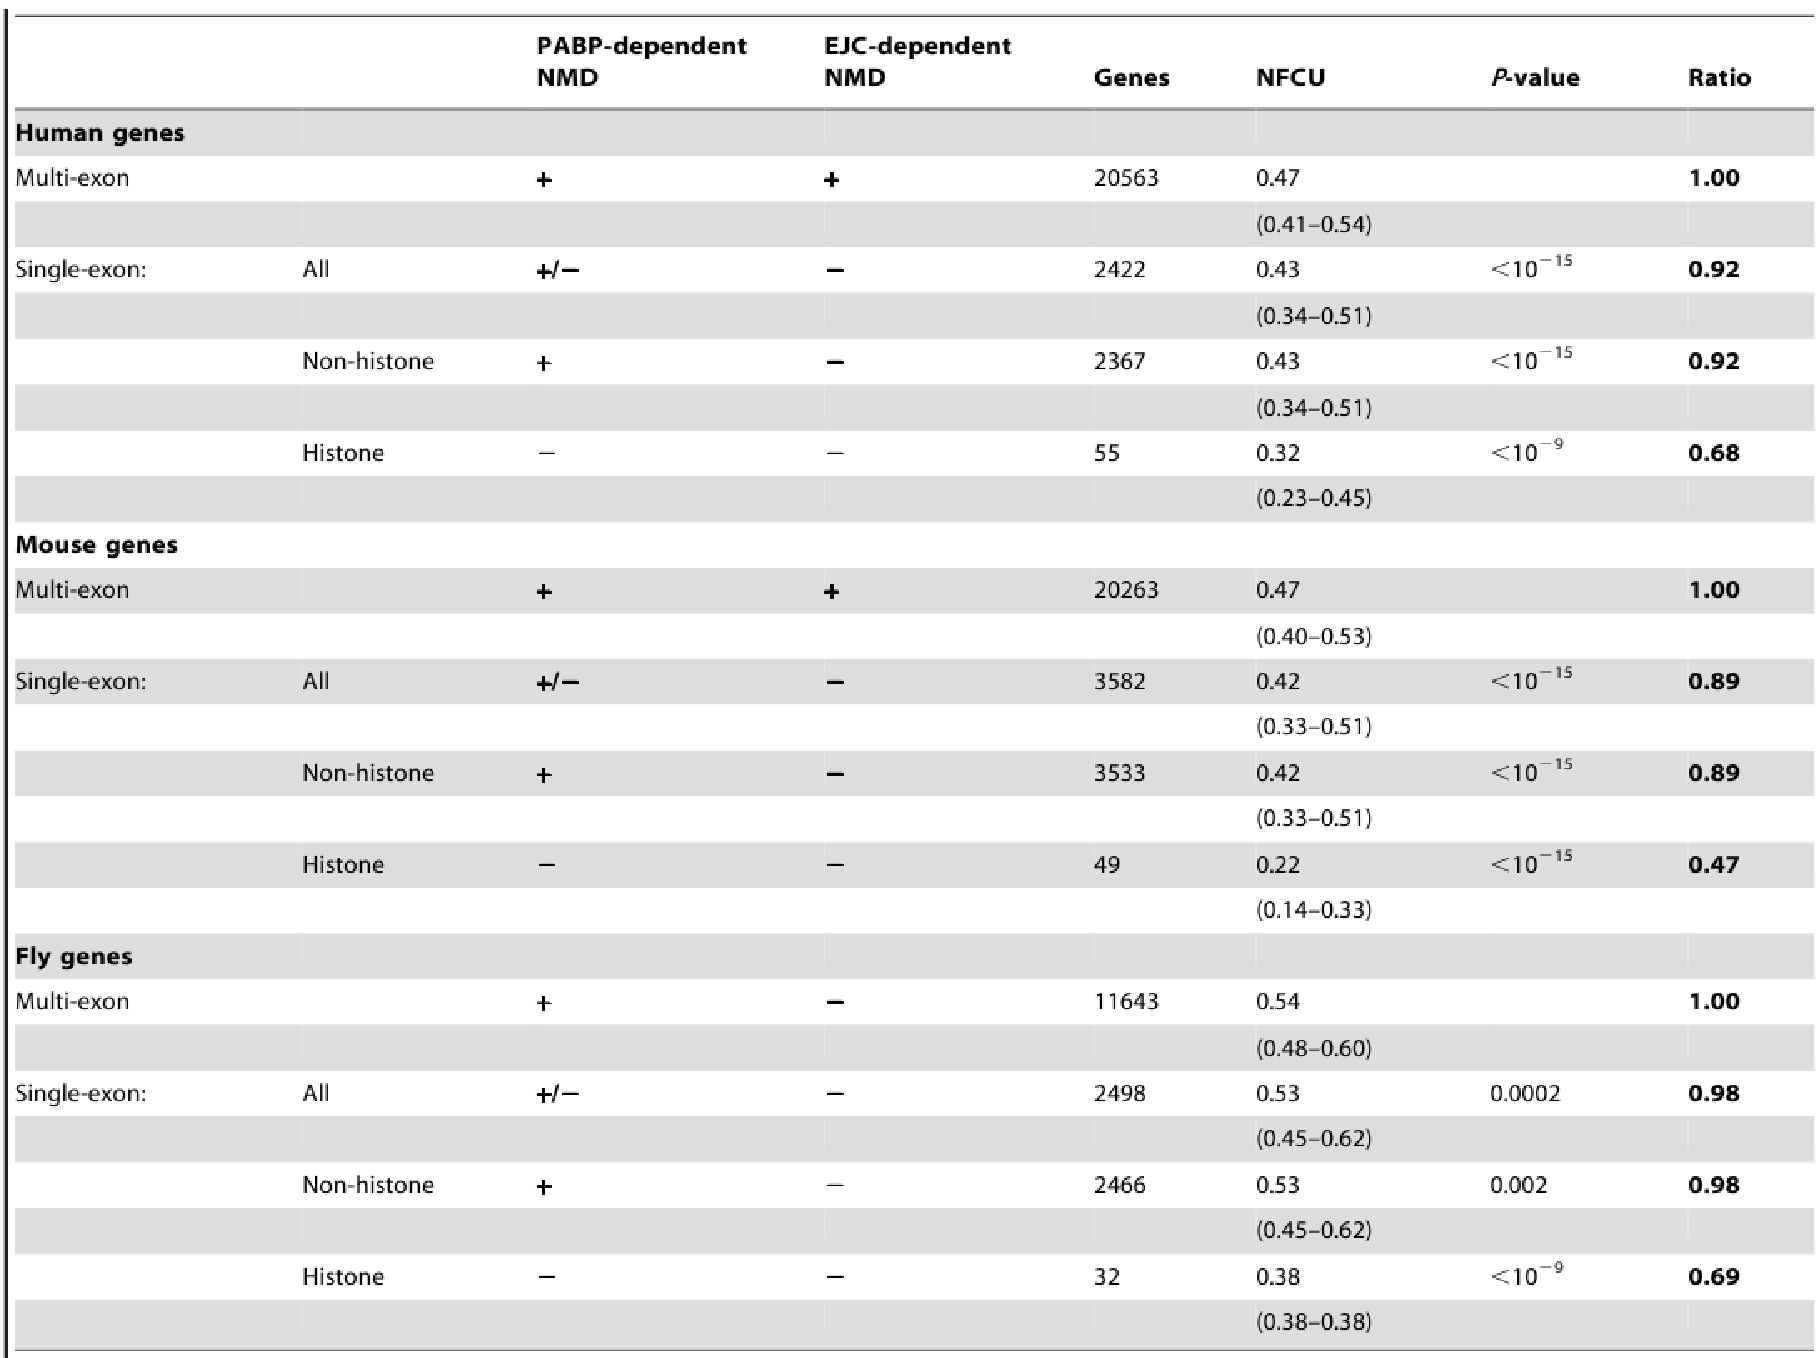
\includegraphics{rys6.pdf}}\\
\end{center}
\end{frame}

%slajd 11
\begin{frame}
\begin{center}
\scalebox{0.35}{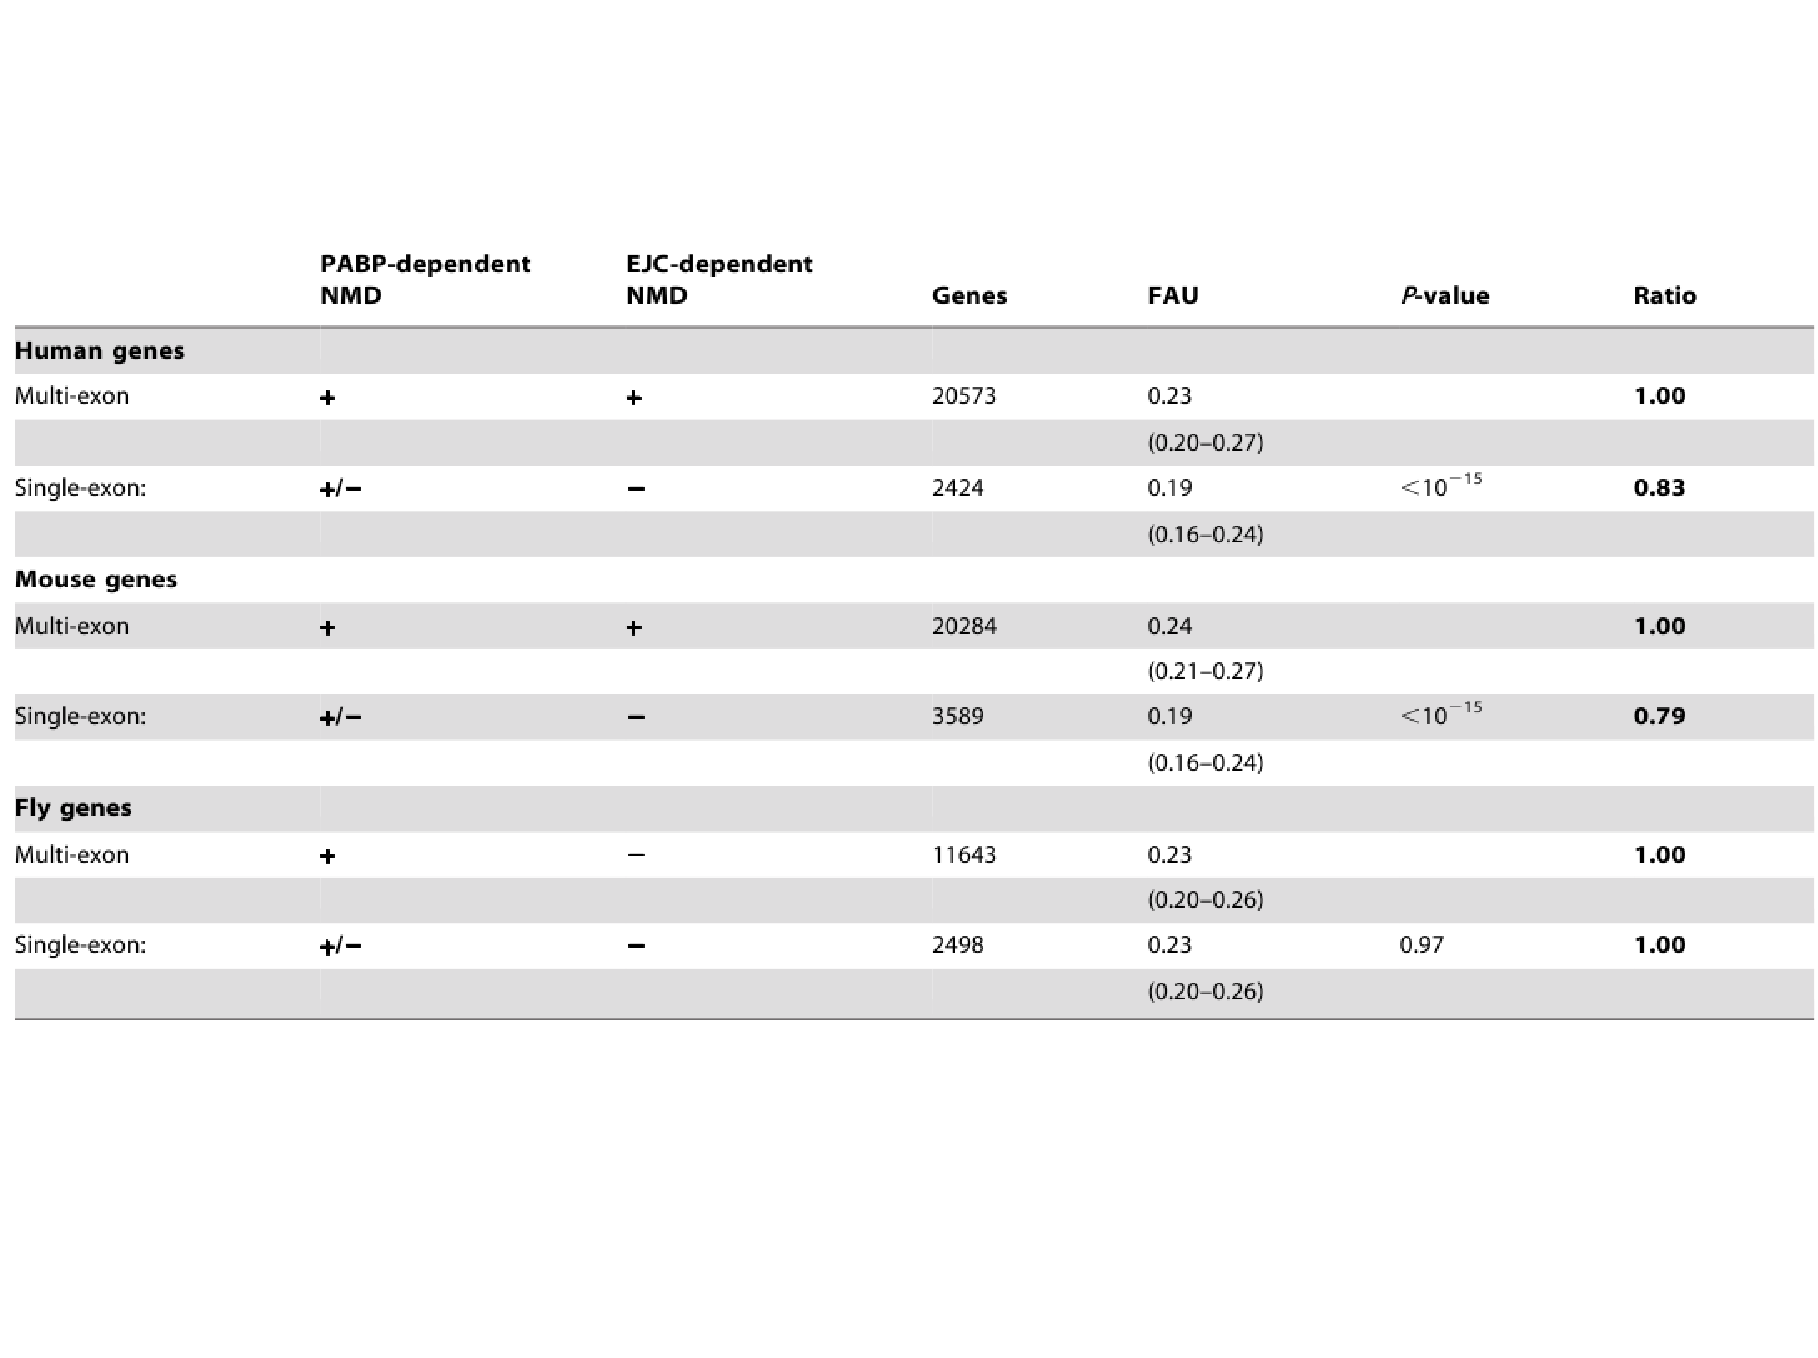
\includegraphics{rys7.pdf}}\\
\end{center}
\end{frame}

%slajd 12
\begin{frame}
\begin{center}
\scalebox{0.35}{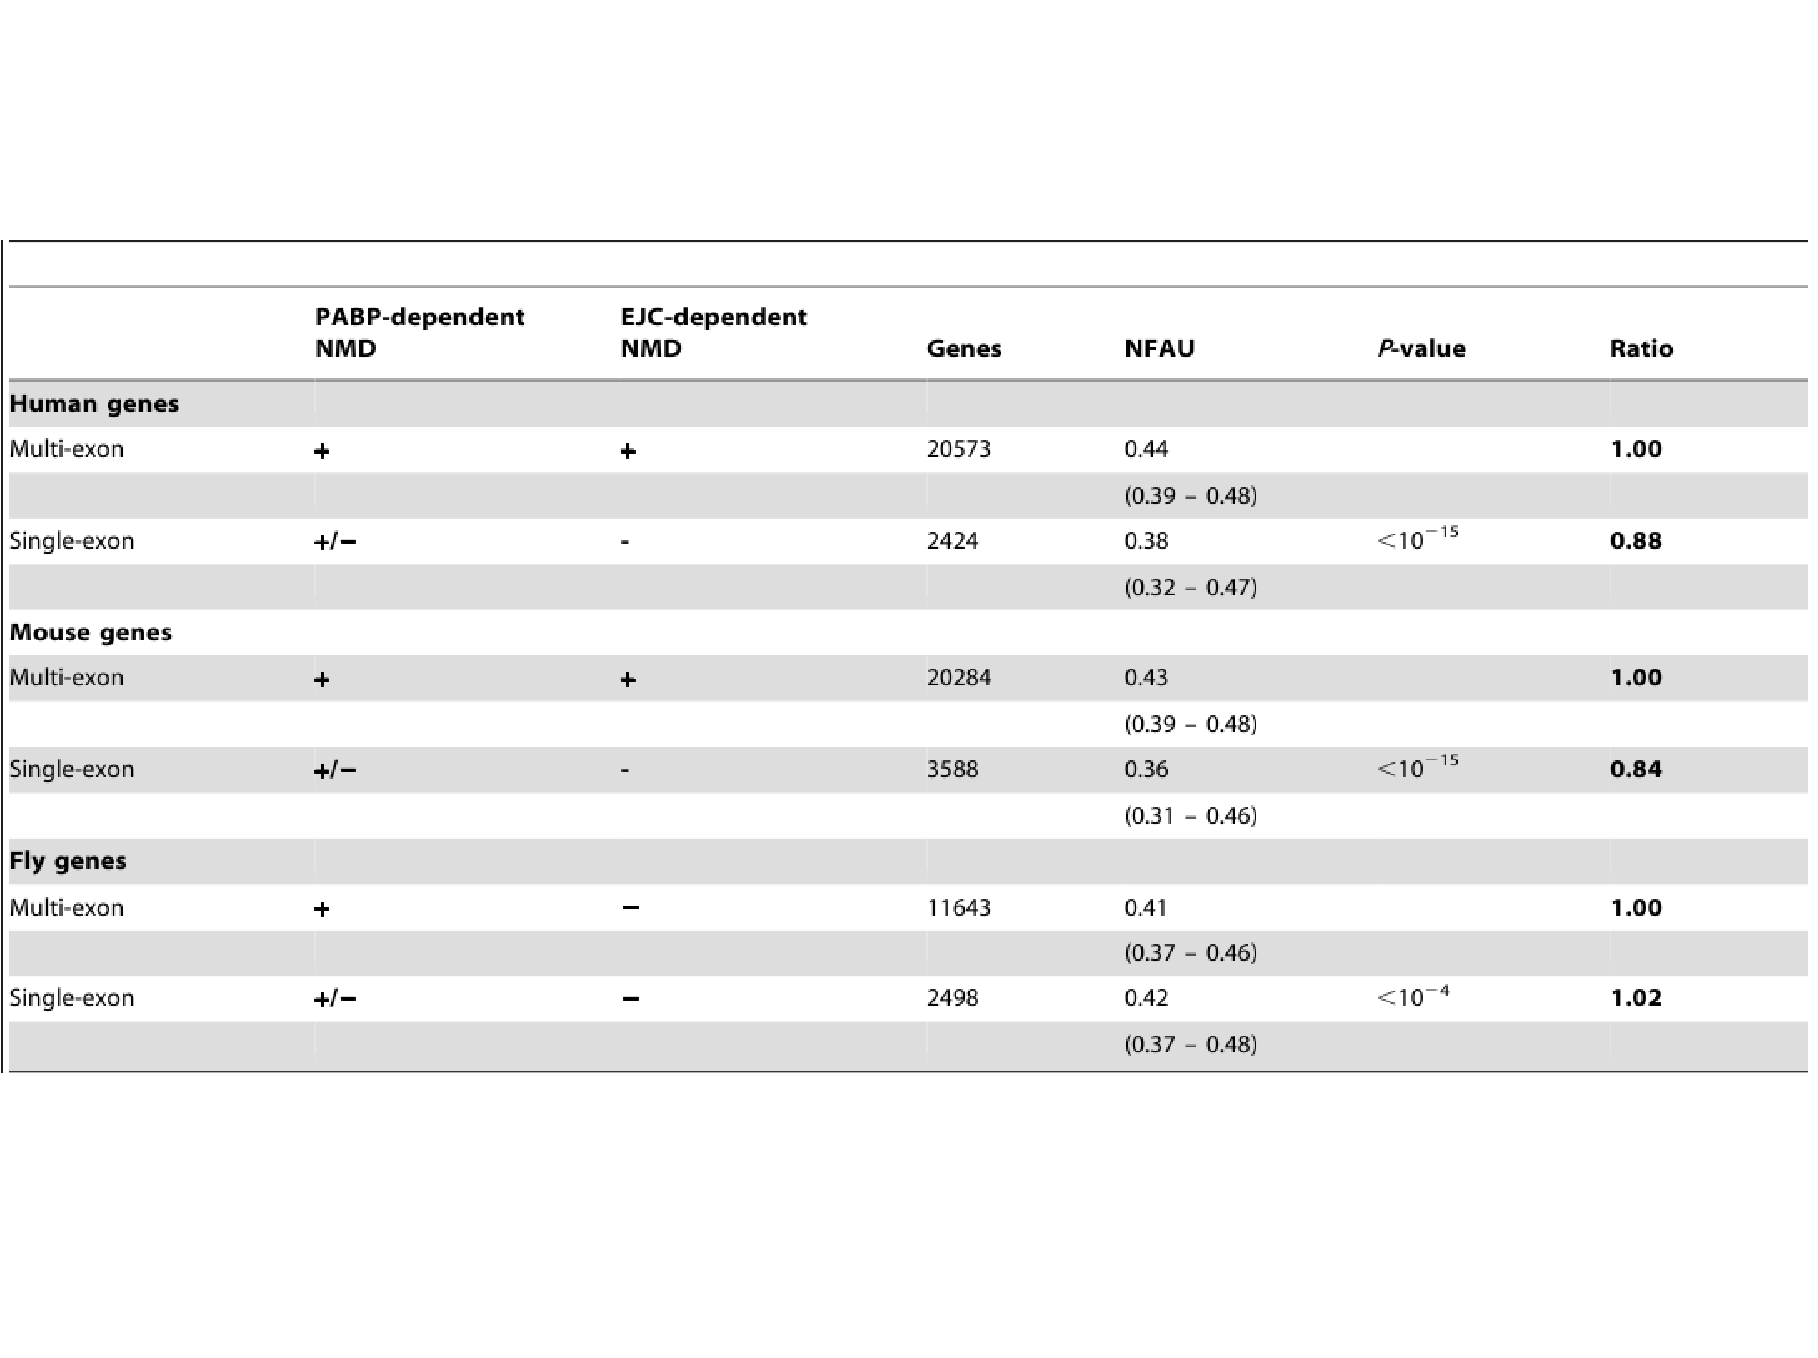
\includegraphics{rys8.pdf}}\\
\end{center}
\end{frame}

%slajd13
\begin{frame}{Dodatkowe wnioski:}
\pause \begin{itemize}
        \item dla genów o współczynniku $\frac{K_{a}}{K_{s}} \sim$  1 organizm obniża
zawartość ryzykownych kodonów i aminokwasów;
\pause \item  $\frac{K_{a}}{K_{s}} \sim$ 0 różnice mogą się akumulować tyklo na poziomie używalności kodonów (selekcja na poziomie aminokwasów);
\pause \item FCU i NFCU w pojedynczo egzonowych i wieloegzonowych genach jest niezależna od kodonów optymalnych;
\pause \item w ostatnim egzonie w wieloegzonowych genach jest o 8$\%$ mniejsze FCU niż w całości (7$\%$ u myszy, bez różnic u muchy) 
       \end{itemize}
\end{frame}

%slajd 14
\begin{frame}
\begin{block}{Metoda 1}
Badanie rozkładów kodonów tylko dla aminokwasów z kodonami ryzykownymi i poczwórnie zdegenerowanych
(leucyna,seryna,arginina i glicyna).
\end{block}
\tiny{
 ,,The usage of codons which are similar to stop codons in the genomes of {\it Xylella fastidiosa} and 
''\\
D.~Galves-dos-Santos i współ.,2011, {\it  Curr Microbiol} 62, 1090-1095
}
\end{frame}

%slajd 15
\begin{frame}
\begin{center}
\scalebox{0.4}{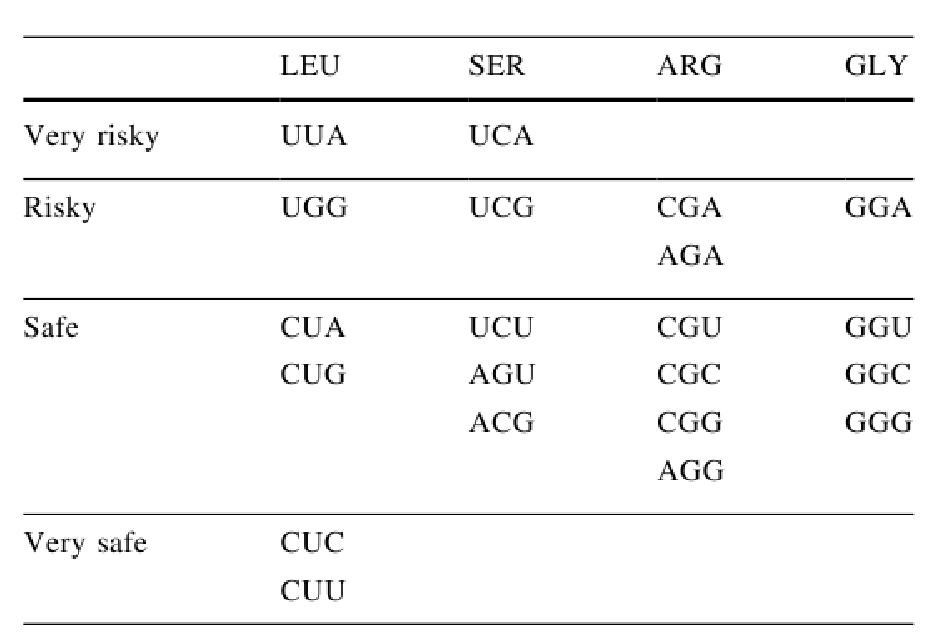
\includegraphics{rys9.pdf}}\\
\end{center}
\end{frame}{\it Xanthomonas citri}

%slajd 16
\begin{frame}
\begin{center}
\scalebox{0.35}{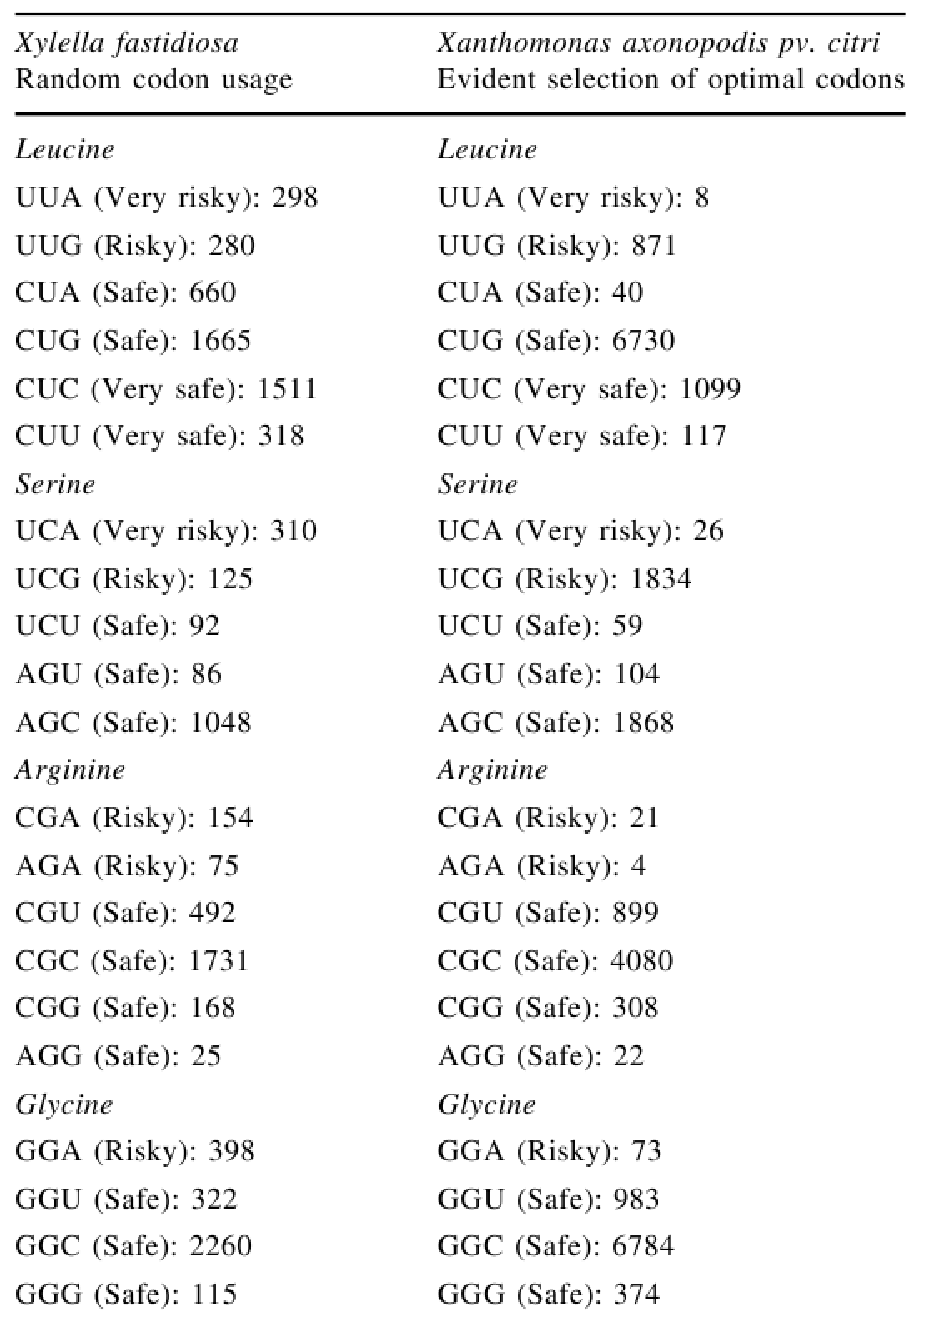
\includegraphics{rys10.pdf}}\\
\end{center}
\end{frame}

%slajd 17
\begin{frame}
\begin{center}
\scalebox{0.35}{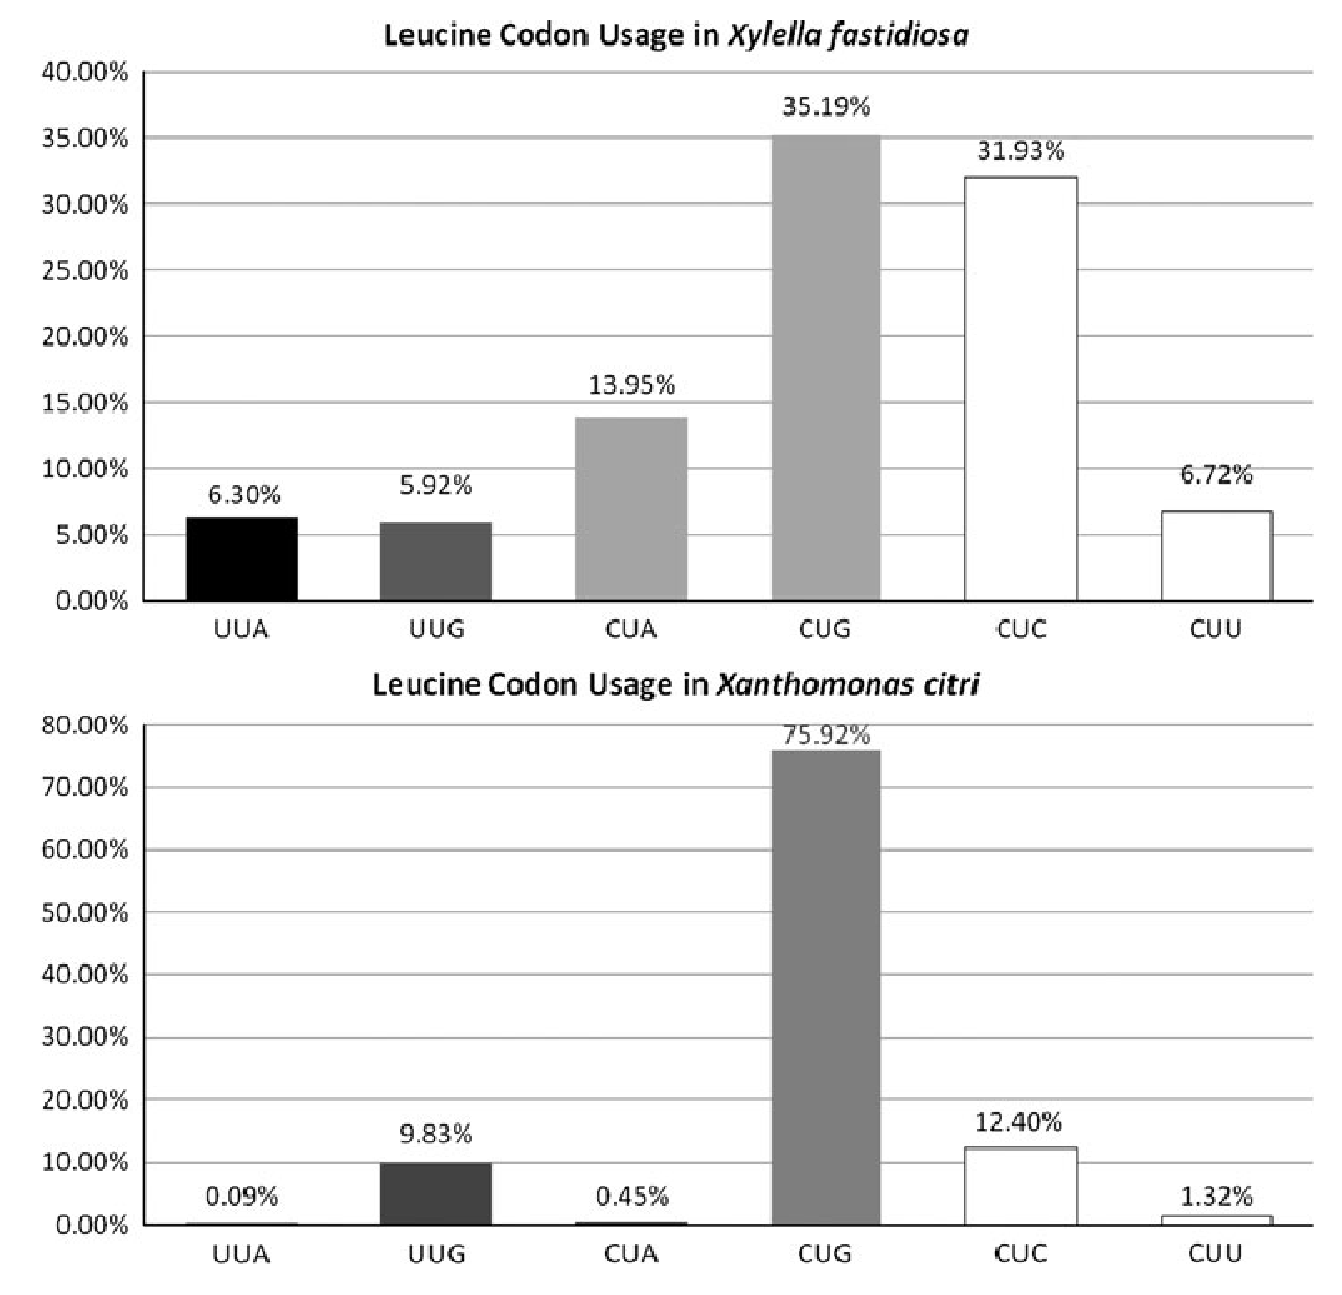
\includegraphics{rys11.pdf}}\\
\end{center}
\end{frame}

%slajd 18
\begin{frame}
\begin{center}
\scalebox{0.35}{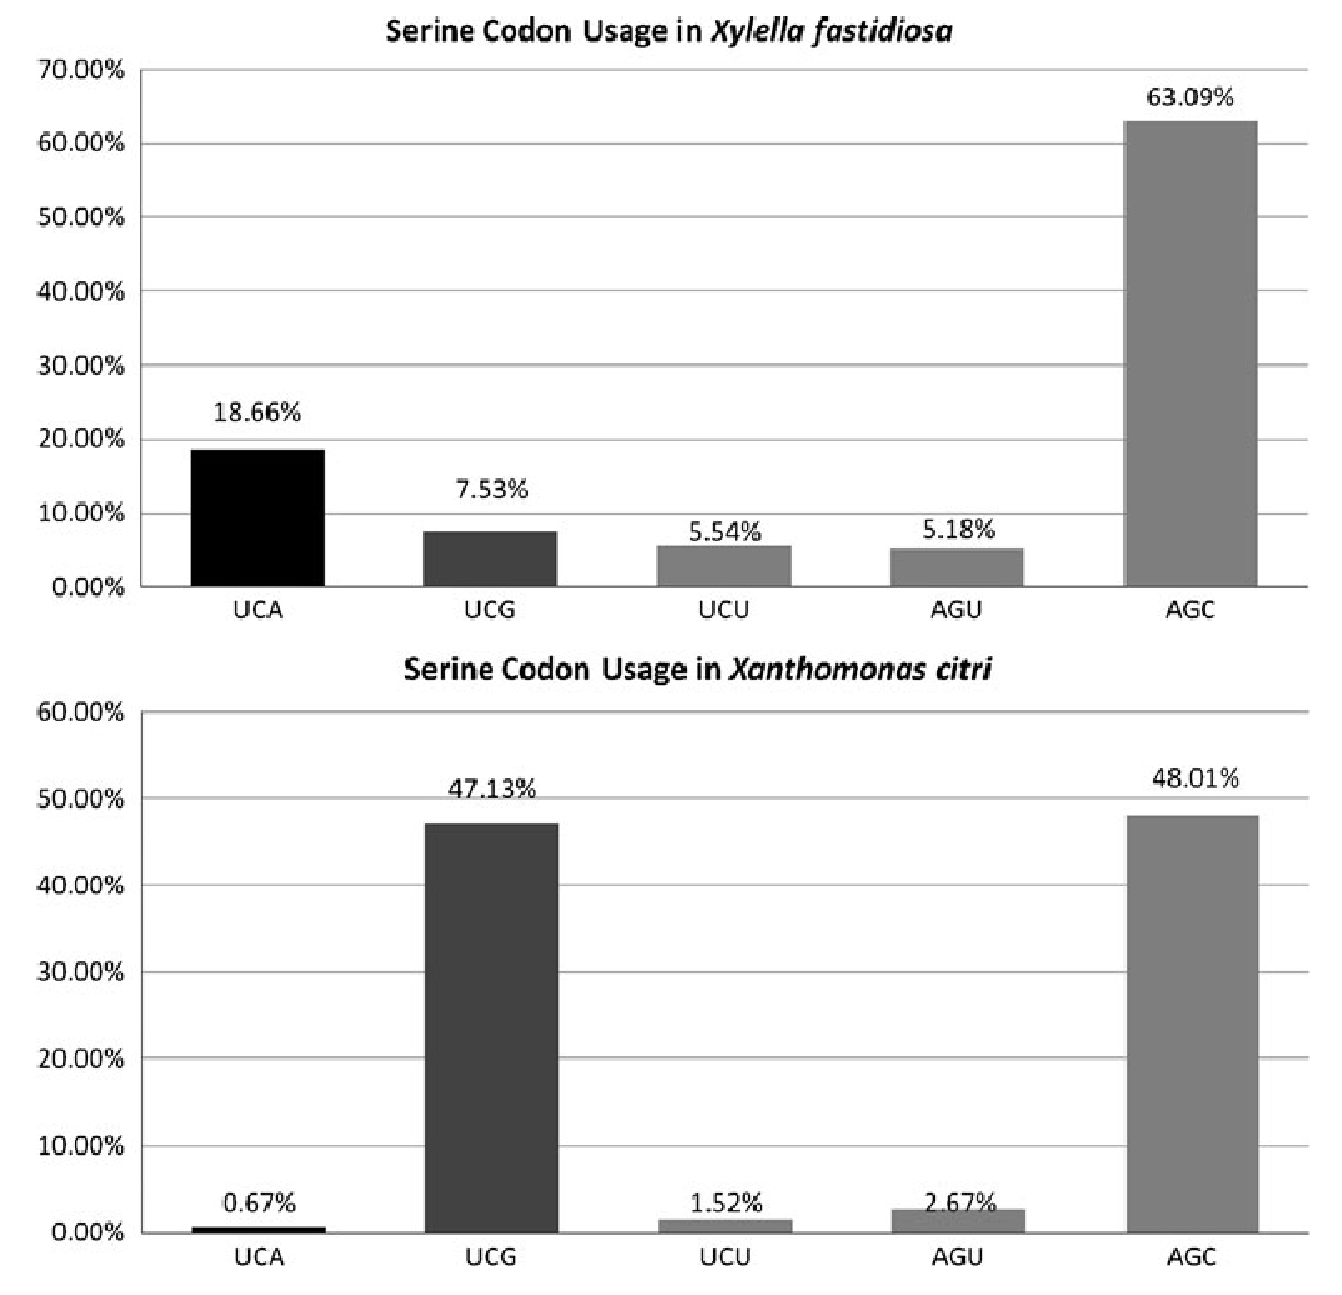
\includegraphics{rys12.pdf}}\\
\end{center}
\end{frame}

%slajd 19
\begin{frame}
\begin{itemize}
 \item założenie, że {\it Xylella fastidiosa} (wolno rosnąca) używa losowo kodonów wynika
z częstszego używania kodonów bardzo ryzykownych niż {\it Xanthomonas citri} (szybko rosnąca).
\pause \item 
\end{itemize}
\end{frame}

%slajd 20
\begin{frame}{Używalność kodonów ryzykownych dla bazy prokaryotów}
\begin{block}{Materiały}
 Do analizy została wzięta baza genomów prokaryotów oprócz {\it Mycoplasmy}
 ze względu na różnice w kodzie genetycznym. Analiza używalności została 
wykonana na zbiorach sekwencji kodujących bialko z i bez sekwencji kodujących
 białka rybosomalne.
\end{block}
\pause
\begin{block}{Metoda}
Dla każdego genomu został wyliczony średni współczynnik FCU, FAU, NFCU, NFAU, NRSCU oraz średnie GC.
\end{block}
\end{frame}

%slajd 18
\begin{frame}
\begin{center}
\scalebox{0.35}{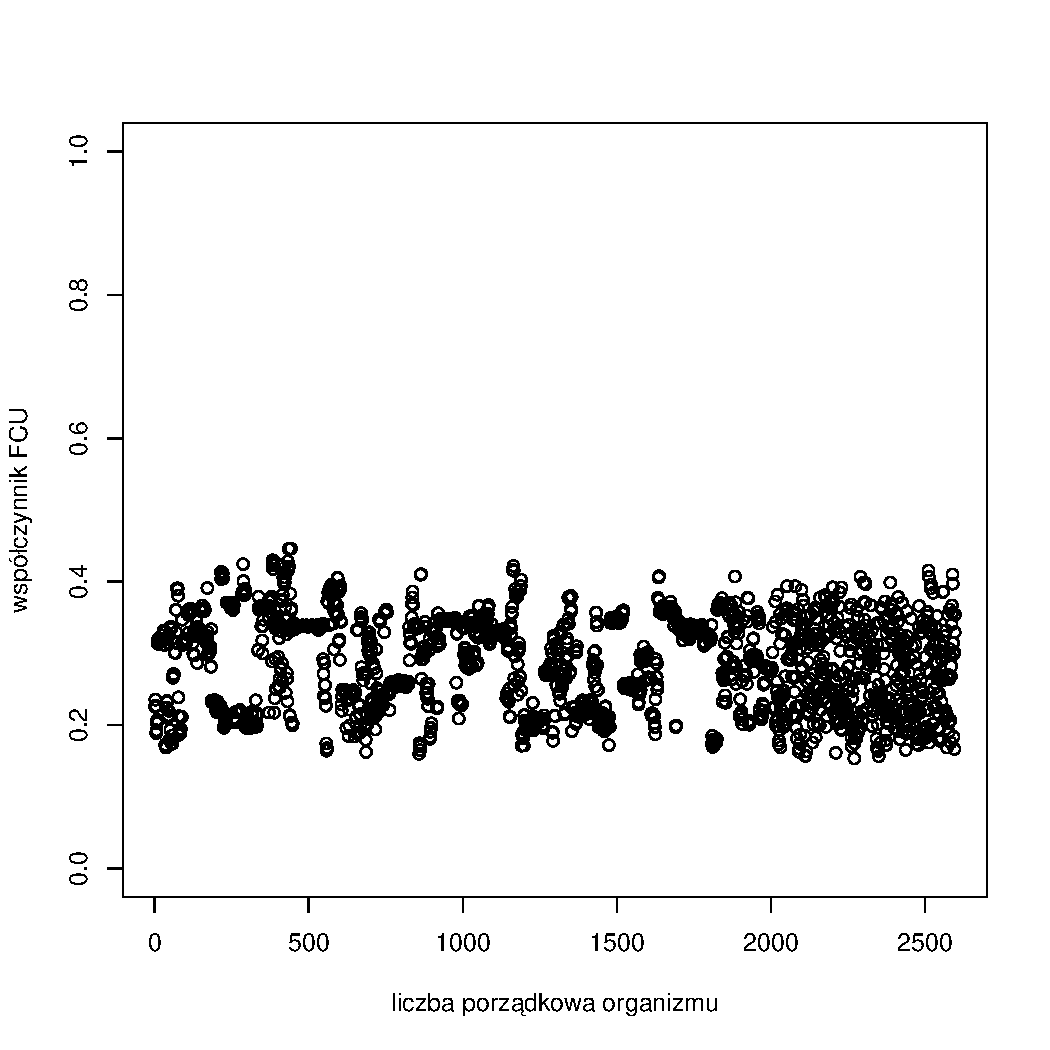
\includegraphics{fc1.pdf}}\\
\end{center}
\end{frame}

\begin{frame}
\begin{center}
\scalebox{0.35}{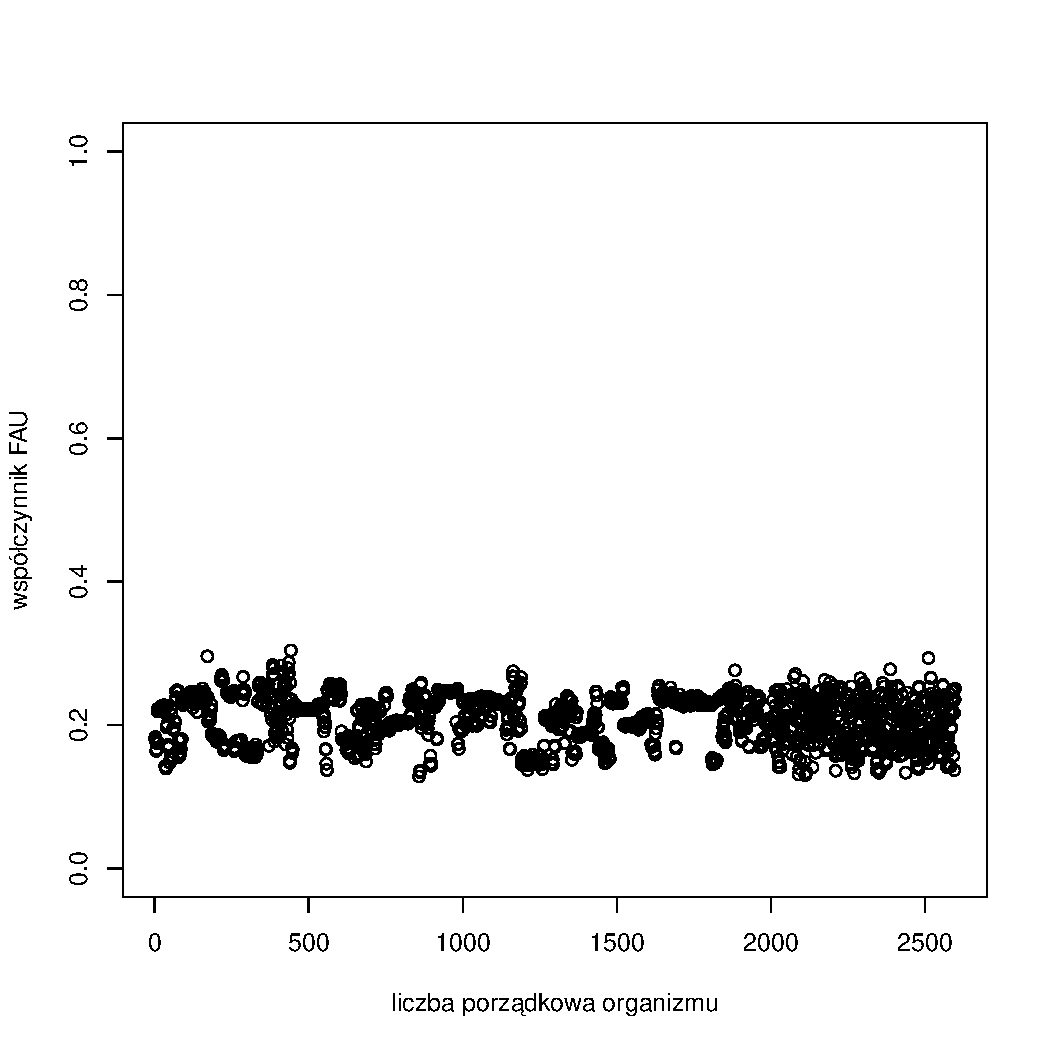
\includegraphics{fc2.pdf}}\\
\end{center}
\end{frame}

\begin{frame}
\begin{center}
\scalebox{0.35}{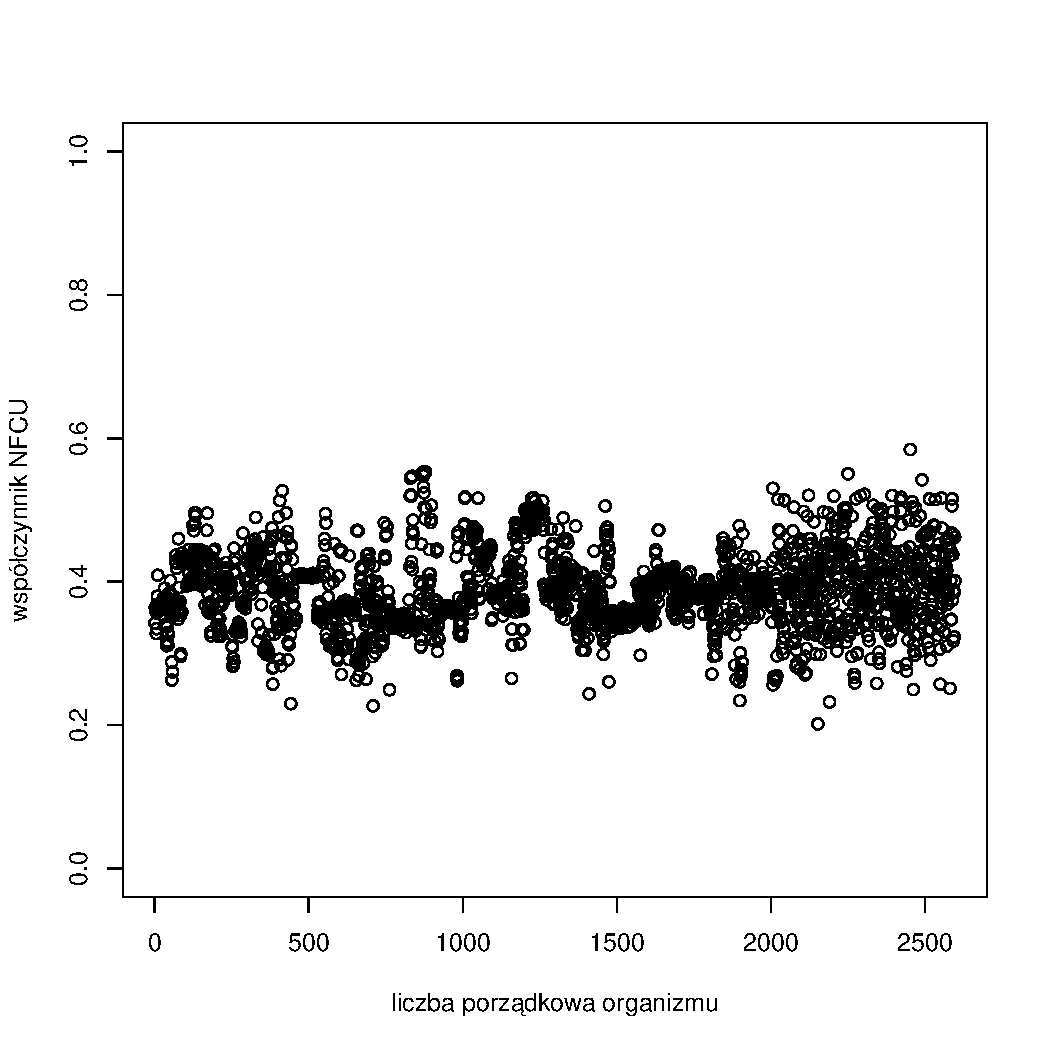
\includegraphics{fc3.pdf}}\\
\end{center}
\end{frame}

\begin{frame}
\begin{center}
\scalebox{0.35}{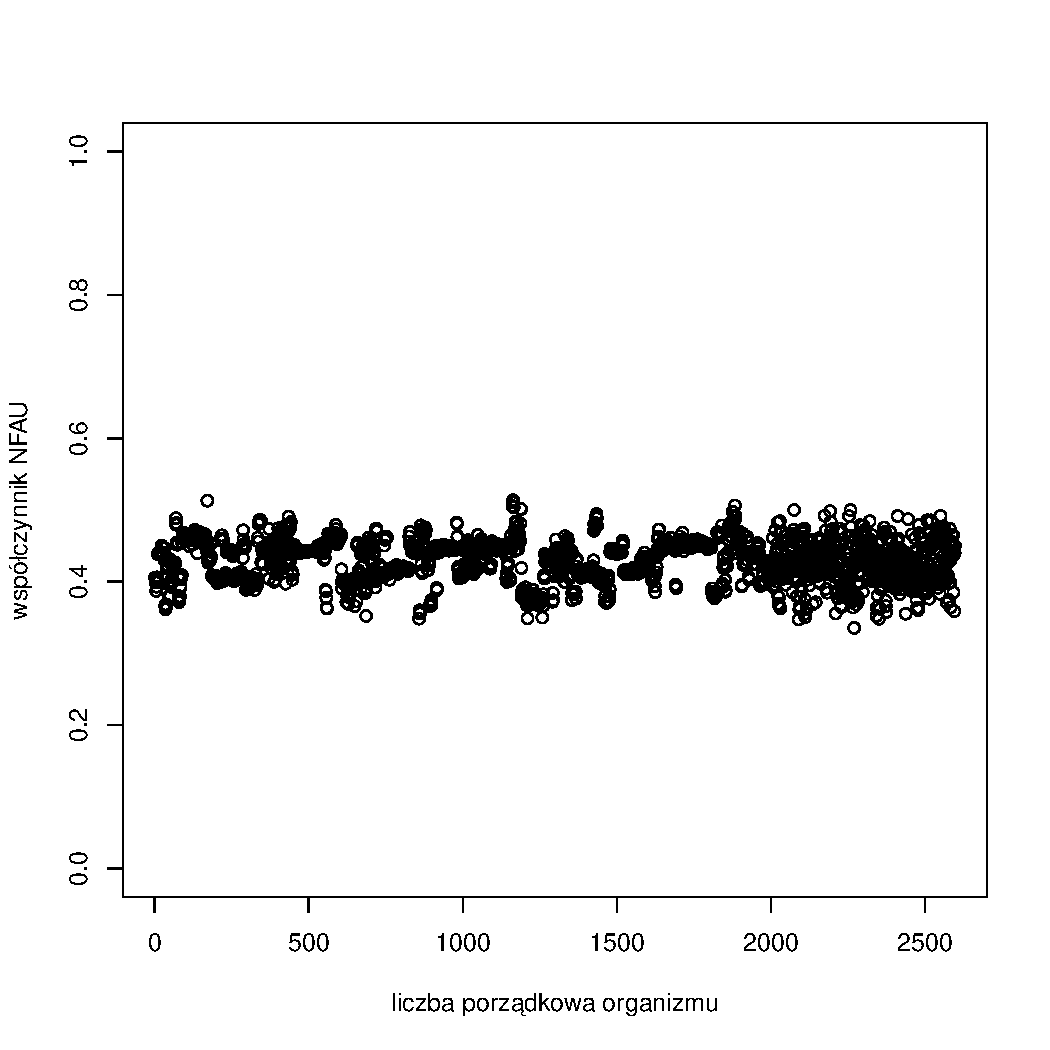
\includegraphics{fc4.pdf}}\\
\end{center}
\end{frame}

\begin{frame}
\begin{center}
\scalebox{0.35}{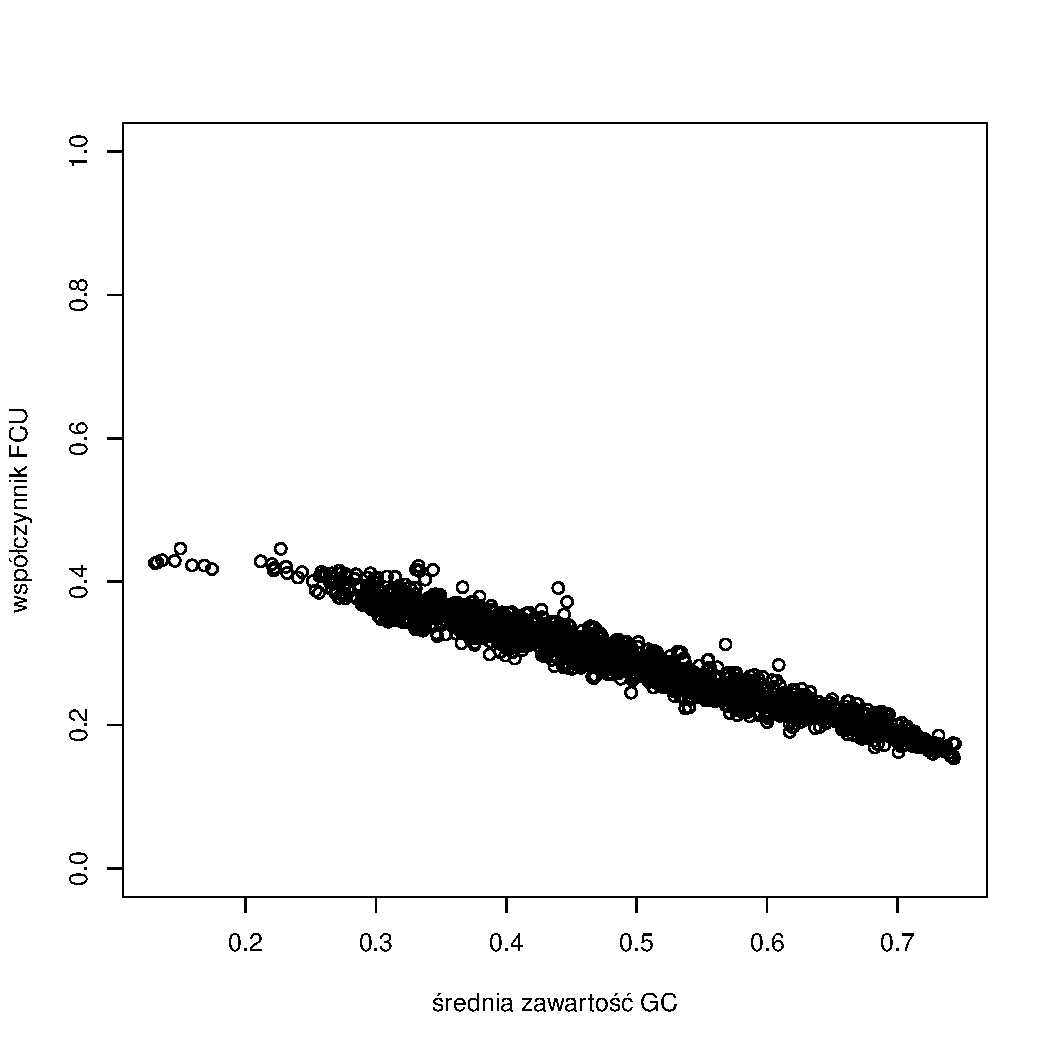
\includegraphics{fc5.pdf}}\\
\end{center}
\end{frame}

\begin{frame}
\begin{center}
\scalebox{0.35}{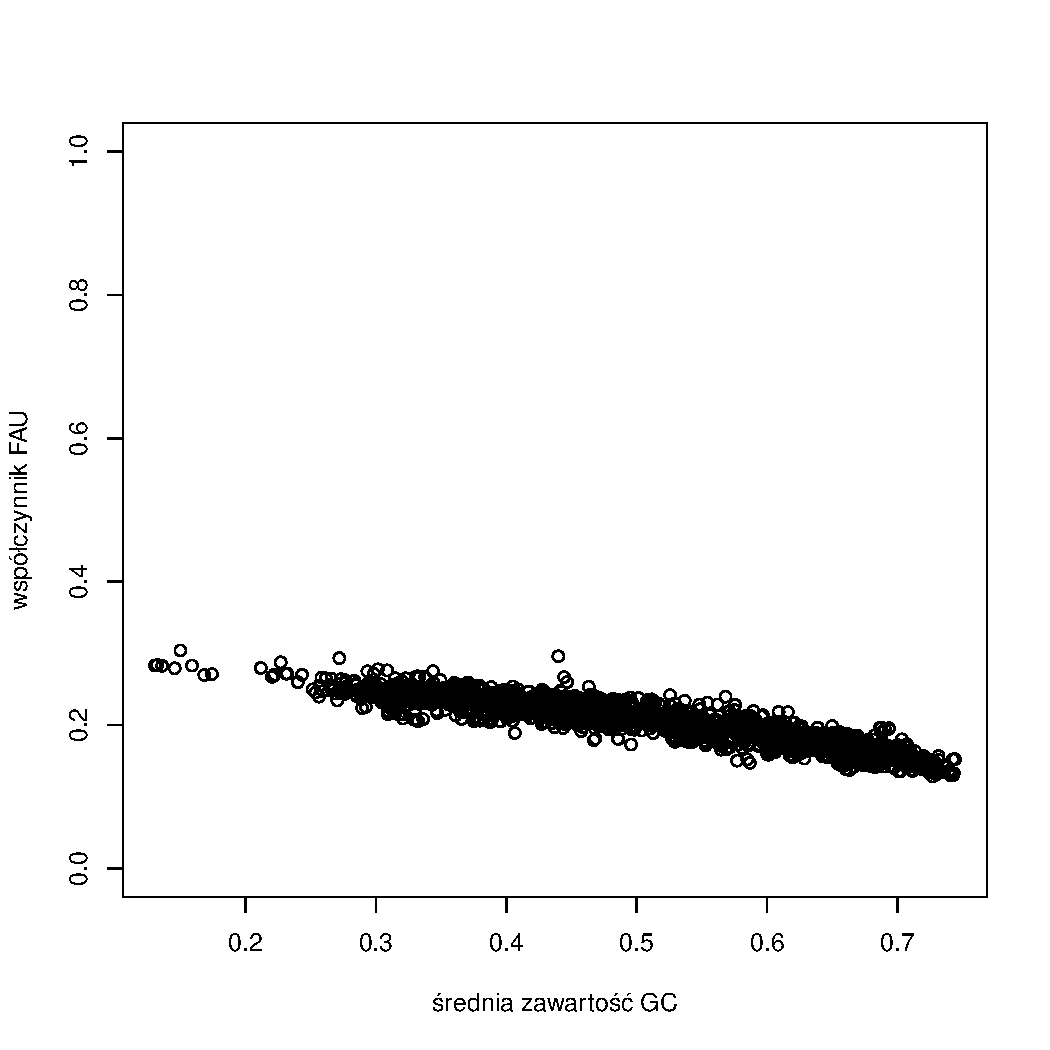
\includegraphics{fc6.pdf}}\\
\end{center}
\end{frame}

\begin{frame}
\begin{center}
\scalebox{0.35}{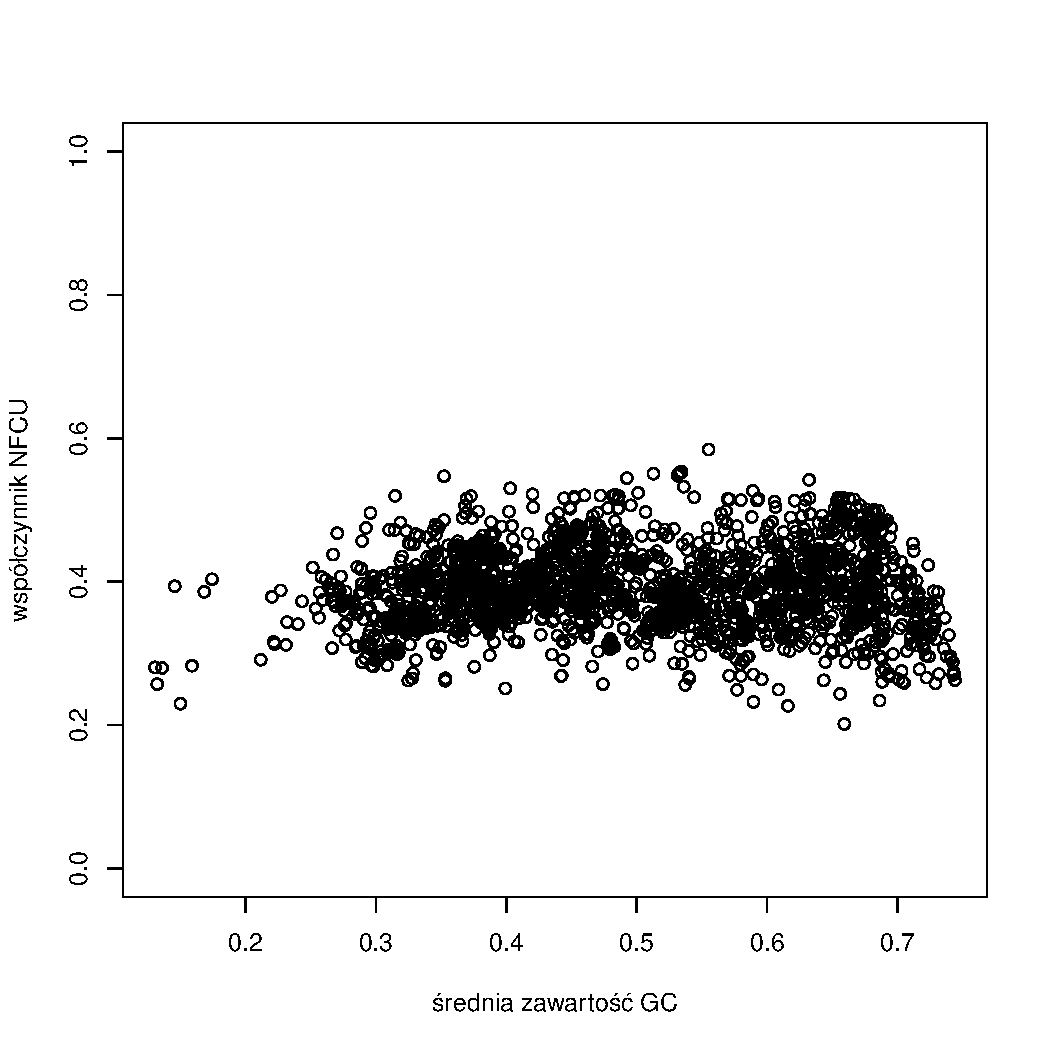
\includegraphics{fc7.pdf}}\\
\end{center}
\end{frame}

\begin{frame}
\begin{center}
\scalebox{0.35}{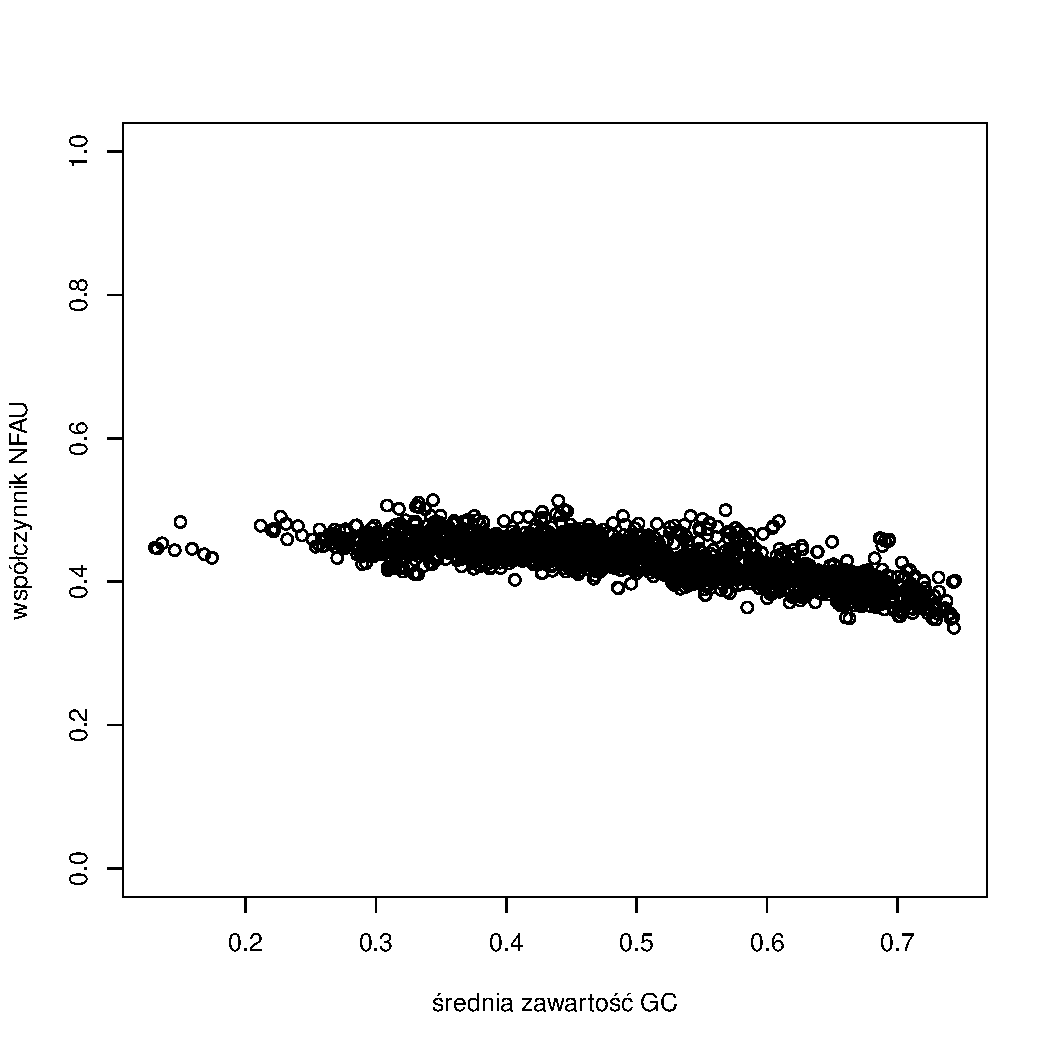
\includegraphics{fc8.pdf}}\\
\end{center}
\end{frame}


\begin{frame}
\begin{center}
\scalebox{0.35}{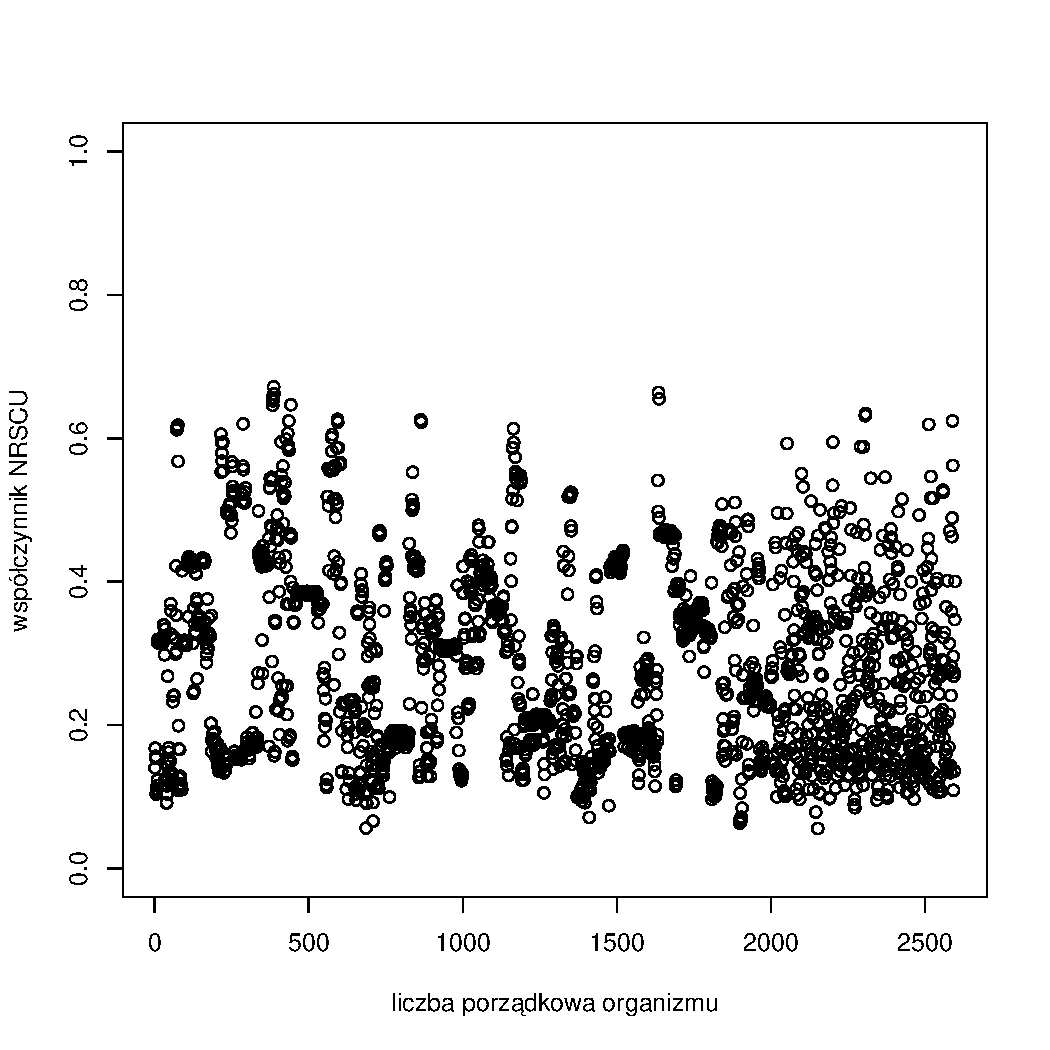
\includegraphics{fc11.pdf}}\\
\end{center}
\end{frame}

\begin{frame}
\begin{center}
\scalebox{0.35}{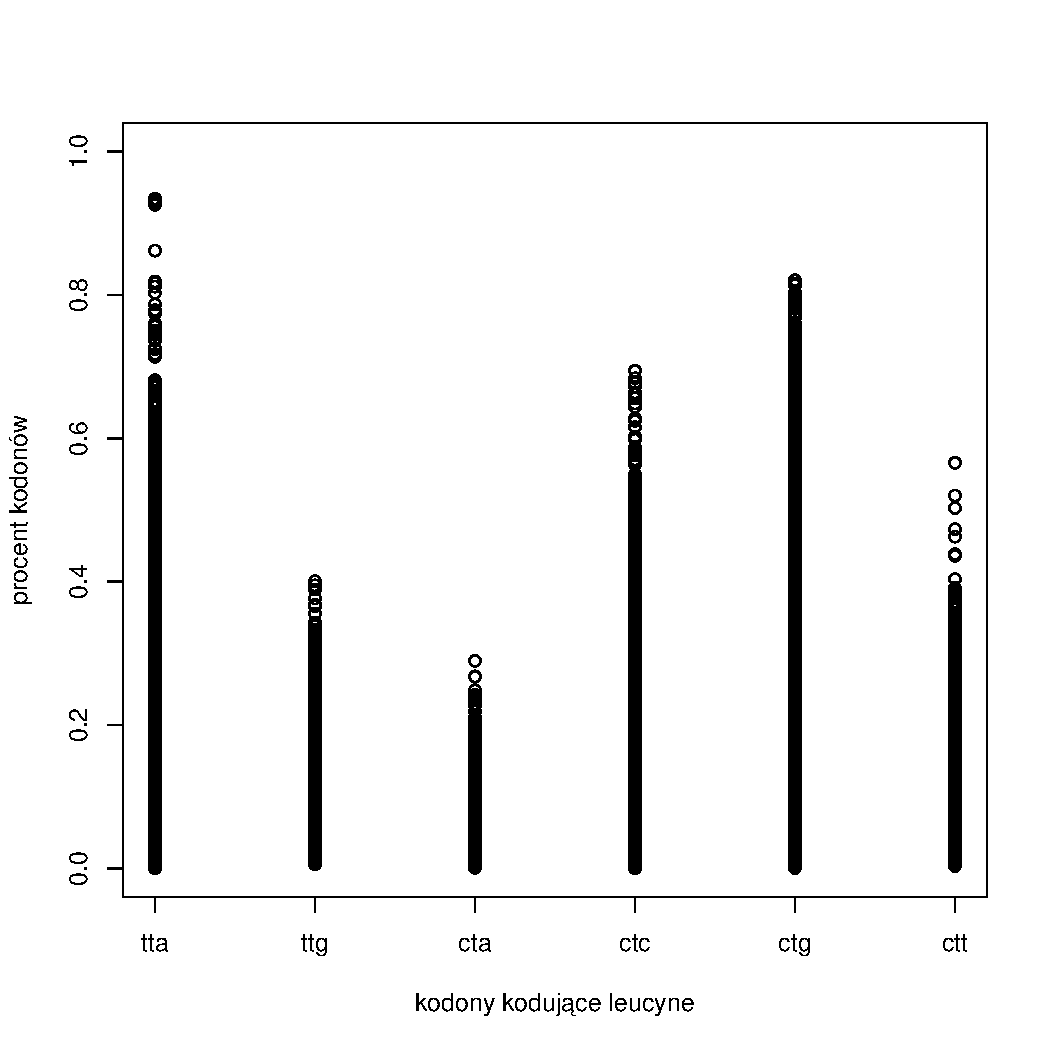
\includegraphics{leucyna.pdf}}\\
\end{center}
\end{frame}

\begin{frame}
\begin{center}
\scalebox{0.35}{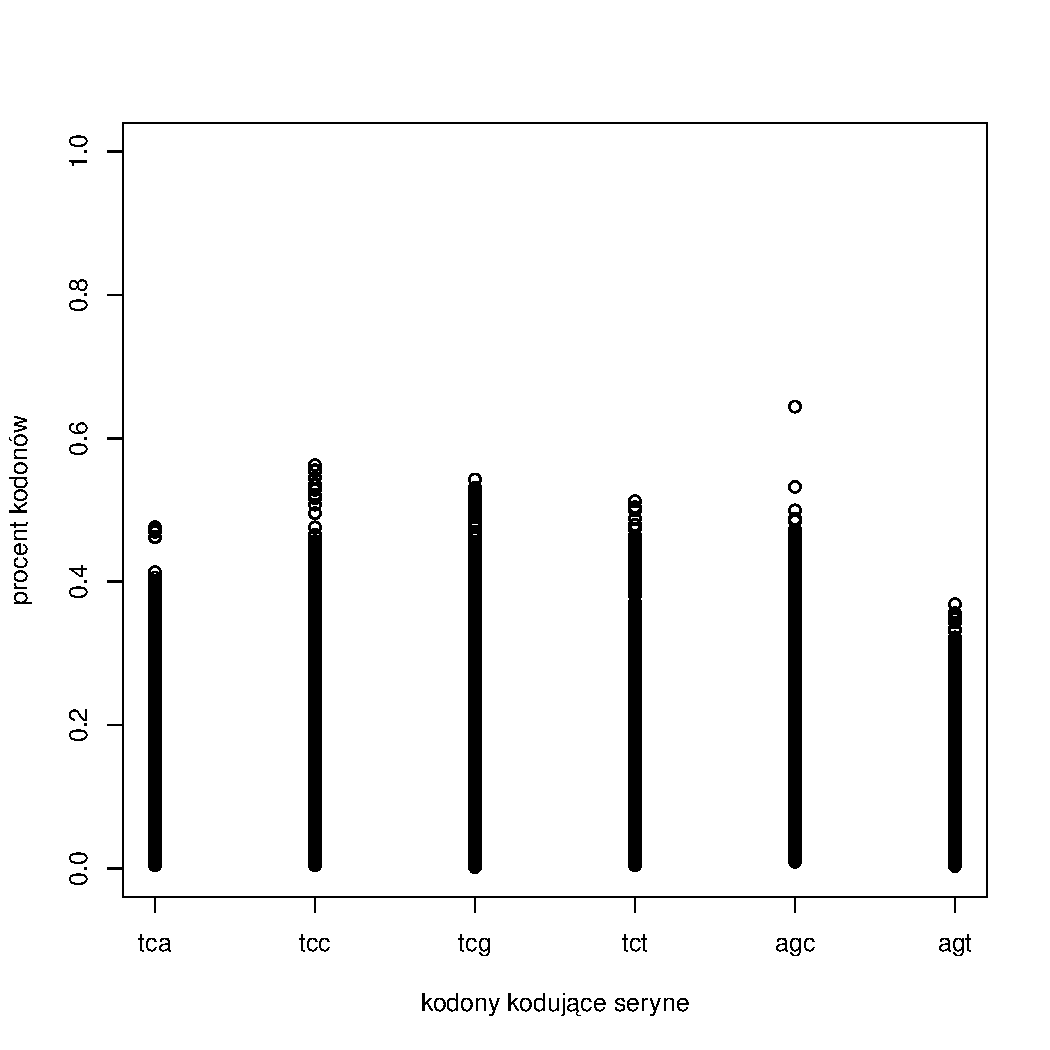
\includegraphics{seryna.pdf}}\\
\end{center}
\end{frame}

\begin{frame}
\begin{center}
\scalebox{0.35}{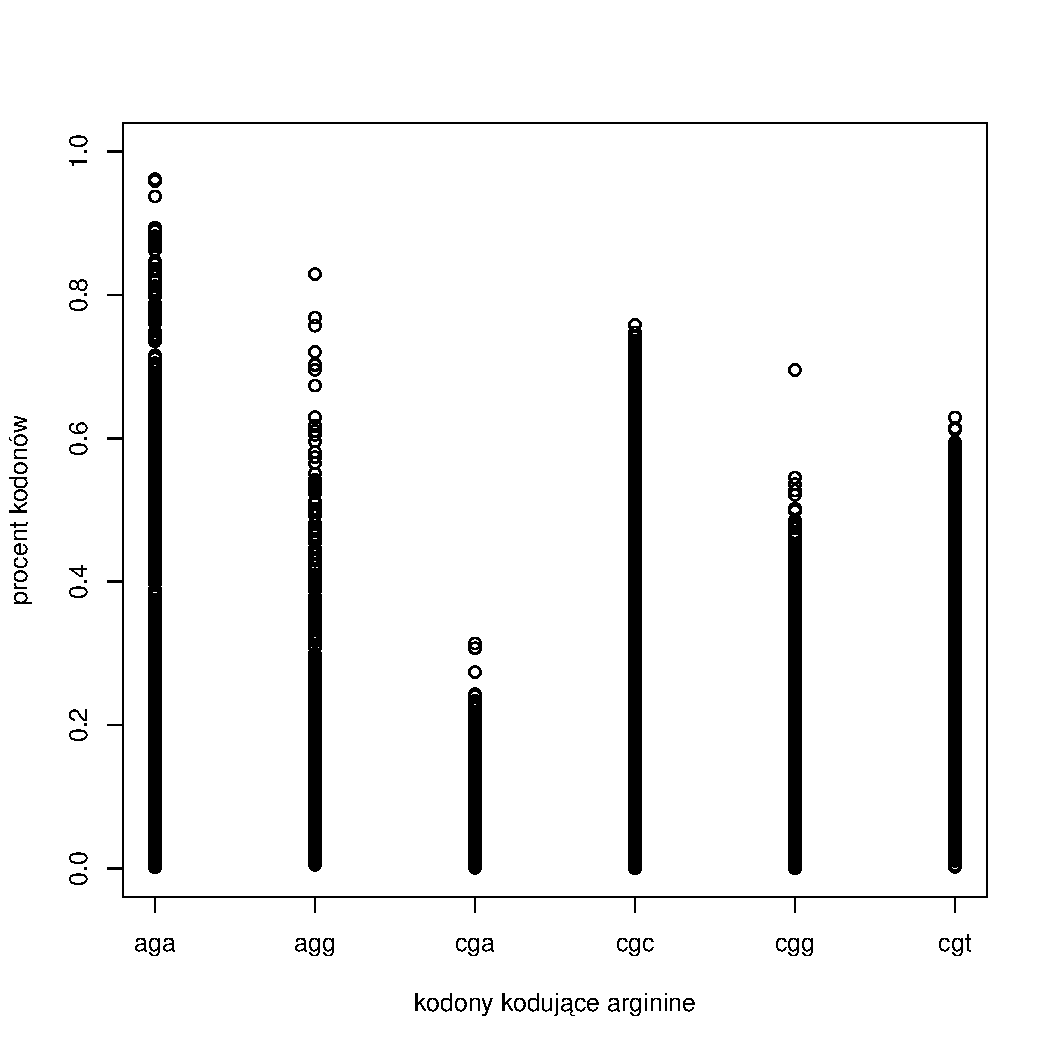
\includegraphics{arginina.pdf}}\\
\end{center}
\end{frame}

\begin{frame}
\begin{center}
\scalebox{0.35}{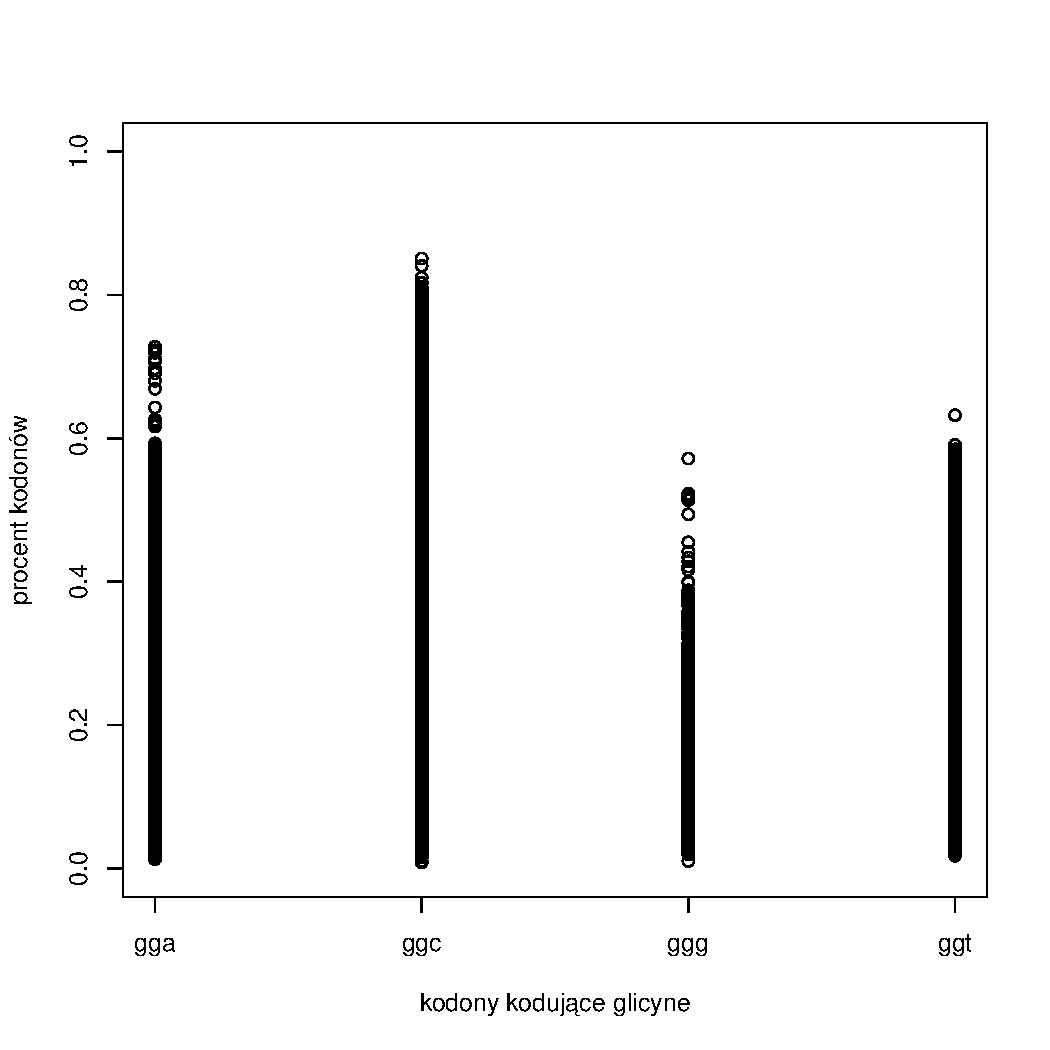
\includegraphics{glicyna.pdf}}\\
\end{center}
\end{frame}
\end{document}

